\documentclass{jcgt}
\usepackage{tikz}
\definecolor{darkgreen}{RGB}{0,192,0}

\setciteauthor{Alan Wolfe}
\setcitetitle{GPU Efficient Texture Based Bezier Curve Evaluation}

% Mark submissions with the date of submission using the following line:
%\submitted{\today}

% Once an article is accepted accepted, switch to the following line and comment the preceding one. The editor will supply the argument values.
\accepted{2014-02-07}{2014-02-07}{2014-02-07}{Editor Name}{3}{1}{1}{1}{2014}
\seturl{http://jcgt.org/published/0003/01/01/}


%%%%%%%%%%%%%%%%%%%%%%%%%%%%%%%%%%%%%%%%%%%%%%%%%


\begin{document}

\usetikzlibrary{arrows.meta}
\tikzset{>={Latex[width=3mm,length=3mm]}}

\title{GPU Efficient Texture Based Bezier Curve Evaluation}

\author
       {Alan Wolfe\\Blizzard Entertainment}

\teaser{
  \begin{tikzpicture}[x=5in,y=1.7in]
    \node[anchor=south west,inner sep=0] at (0,0) {
\includegraphics[width=5in,height=1.7in]{Teaser.png}};
    % representative line for where the quadratic bezier curve lives in the bilinear sampled texture
    \draw[yellow,->,line width=0.5mm]    (0.41,0.25) -- (0.58,0.75);
    \draw (0.08,0.25) node[] {\Huge{A}};
    \draw (0.25,0.25) node[] {\Huge{B}};
    \draw (0.08,0.75) node[] {\Huge{B}};
    \draw (0.25,0.75) node[] {\Huge{C}};    
  \end{tikzpicture}
  \caption{Left: 2x2 texture containing control points for a quadratic Bezier curve per color channel. Middle: The texture as viewed with bilinear sampling. Right: The resulting curves when sampling along the yellow line (Alpha curve omitted).}
  \label{fig:teaser}
}

\maketitle
\thispagestyle{firstpagestyle}

\begin{abstract}
\small
Modern graphics techniques expose internal parameters to allow re-use and to help seperate the technical implementation from the artistic usage cases.  A popular choice is to expose parameters as a customizable curve and to quantize the curve into a texture which either leads to lower quality results, or more texture memory being used to accomodate a higher sampling frequency.  The technique presented in this paper leverages the capabilities of GPU texture samplers to allow more efficient storage and evaluation of both integral and rational Bezier curves of any order, resulting in higher fidelity for the same costs.  Piecewise curves, B-Splines and Nurbs are mentioned, and there are also limited applications towards vector graphics.
\end{abstract}


%-------------------------------------------------------------------------
\section{Introduction}
\label{sec:introduction}
There are two basic ways for a shader program to gain access to customized curve data.  One way is to evaluate the curve on the CPU at discrete intervals and put those points into a texture that can be used by the GPU.  The other way is to pass curve control point data from the CPU to the shader program as shader constants.

Baking curve points into a texture means that the shader program doesn't need to know what type of curve it was that made the data, but comes at the loss of quality since there are a finite number of curve points sampled, and the data between points is just a linear interpolation between the samples.  If higher quality is desired, you can achieve this by increasing the resolution of the texture to be able to trade accuracy for texture memory.

Passing control point data to a shader program as shader constants allows you to get high quality curve calculations, but comes at the cost of the shader program being written in a very specific way for the type of curve you want to use, as well as more shader program instructions to calculate specific curve points.

\begin{figure}
  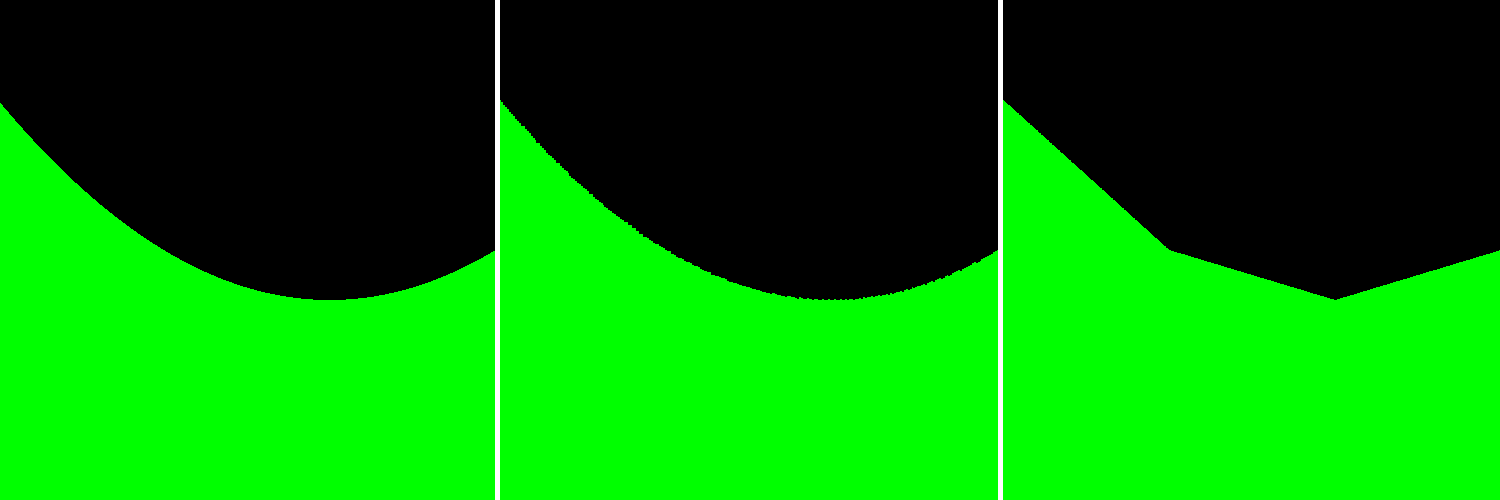
\includegraphics[width=5in]{Figure2.png}
  \caption{Left: A quadratic Bezier curve written to the green channel, and it's baked out equivelant using 4 pixels written to the red channel.  Right: The technique from this paper also using 4 pixels, written to the green channel, and the baked out equivelant written to the red channel again for comparison. \label{fig:sampleconfig}}
  \label{fig:quickcomparison}
\end{figure}

This paper shows a third method where:
\begin{itemize}
  \item Curve data is encoded within a texture in such a way to allow the texture sampler to evaluate polynomial basis functions before the data reaches the shader program.
  \item It gives accuracy results closer to that of shader constant curves, while having less calculation overhead.
  \item The technique can support both integral and rational Bezier curves of any order and can also be used for piecewise curves.
  \item The curve type must be decided on in advance, like when using the shader constant method.
  \item There are limited applications towards vector graphics.
\end{itemize}

A quick comparison of the visual quality of these three techniques can be seen in \autoref{fig:quickcomparison}.

TODO: make those bullet points reference forward into sections of the paper

%-------------------------------------------------------------------------
\section{The Technique}
\label{sec:thetechnique}

The core of this technique is that the linear texture interpolation capabilities on the GPU can be mathematically equivelant to De Casteljeau's algorithm for evaluating Bezier curves.

A one dimensional texture with linear sampling results in the evaluation of a linear Bezier curve (order 1), a two dimensional texture with linear sampling can result in a quadratic bezier curve (order 2), and a three dimensional texture (volumetric texture) with linear sampling can result in a cubic Bezier curve (order 3).

The pattern continues for higher dimensionality textures, and curves of lower degrees can be combined to create curves of higher degrees by either continuing De Casteljeau's algorithm in the shader program, or by using the Bernstein form of Bezier curves to combine multiple curve points with fewer operations.

\subsection{Intuition}

The De Casteljeau algorithm shows us that we can find points on a Bezier curve by evaluating a hierarchy of linear interpolations.  For example, a quadratic curve is the linear interpolation between the linear interpolation of {$\overline{AB}$} and {$\overline{BC}$}, using the same time t for each interpolation (\autoref{lst:GLSLDeCasteljeau})

\begin{lstlisting}[caption={GLSL De Casteljeau Algorithm For a Quadratic Bezier Curve}, label={lst:GLSLDeCasteljeau}]
float QuadraticBezier (
  in float t,
  in float A,
  in float B,
  in float C
) {
    return mix(mix(A,B,t), mix(B,C,t), t);
}
\end{lstlisting}

Bilinear interpolation is used when linear sampling is enabled and a texture sample is taking from a 2d texture.  Bilinear interpolation is achieved by linearly interpolating across one axis (say, the X axis) and then interpolating the two results by the other axis (the Y axis).

From this, we have an idea of how to set up the points in our texture so that when performing bilinear sampling (\autoref{fig:decasteljeauBilinear}), that we will get, as output, points on a quadratic bezier curve.

  \begin{figure}
    % bezier curve diagram
    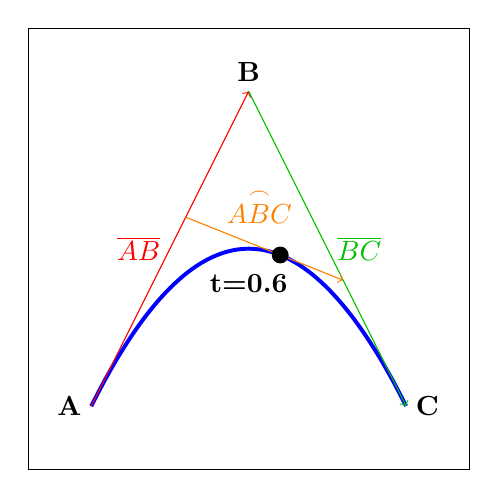
\begin{tikzpicture}[x=4cm,y=4cm]
      % border
      \draw (-0.2,-0.2) -- (1.2,-0.2) -- (1.2,1.2) -- (-0.2,1.2) -- (-0.2,-0.2);
      % 1d quadratic bezier curve with control points 0,1,0
      \draw[scale=1,domain=0:1,smooth,variable=\x,blue,line width=0.5mm] plot ({\x},{2*\x-2*\x*\x});    
      % control polygon / labels
      \draw[red,->]       (0.0,0.0) -- (0.5,1.0);
      \draw[darkgreen,->] (0.5,1.0) -- (1.0,0.0);
      \draw[red]          (0.25,0.5) node[anchor=east] {$\overline{AB}$};
      \draw[darkgreen]    (0.75,0.5) node[anchor=west] {$\overline{BC}$};
      % control point labels
      \draw (0.0,0.0) node[anchor=east]  {\bf{A}};
      \draw (0.5,1.0) node[anchor=south] {\bf{B}};
      \draw (1.0,0.0) node[anchor=west]  {\bf{C}};
      % draw a line from AB->AC for time = 0.75
      \draw[orange,->] (0.3,0.6) -- (0.8,0.4);
      \draw[orange] (0.40,0.55) node[anchor=south west] {$\stackrel{\frown}{ABC}$};
      % draw the point at t=0.6 and label underneath the curve
      \draw[black,fill=black] (0.6,0.48) circle (1mm);
      \draw[black] (0.5,0.45) node[anchor=north] {\bf{t}=0.6};
    \end{tikzpicture}
    % bilinear diagram
    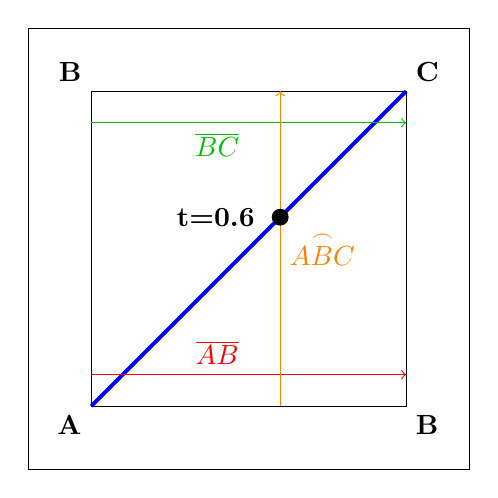
\begin{tikzpicture}[x=4cm,y=4cm]
        % border
        \draw (-0.2,-0.2) -- (1.2,-0.2) -- (1.2,1.2) -- (-0.2,1.2) -- (-0.2,-0.2);
        % box
        \draw (0,0) -- (1,0) -- (1,1) -- (0,1) -- (0,0);
        % representative line for where the quadratic bezier curve lives
        \draw[blue,line width=0.5mm] (0,0) -- (1,1);    
        % corner labels
        \draw (0,0) node[anchor=north east] {\bf{A}};
        \draw (1,0) node[anchor=north west] {\bf{B}};     
        \draw (0,1) node[anchor=south east] {\bf{B}};
        \draw (1,1) node[anchor=south west] {\bf{C}};     
        % x axis interpolation
        \draw[red,->]       (0.0,0.1) -- (1.0,0.1);
        \draw[red]          (0.4,0.1) node[anchor=south] {$\overline{AB}$};
        \draw[darkgreen,->] (0.0,0.9) -- (1.0,0.9);
        \draw[darkgreen]    (0.4,0.9) node[anchor=north] {$\overline{BC}$};
        % y axis interpolation
        \draw[orange,->]    (0.6,0.0) -- (0.6,1.0);
        \draw[orange]     (0.6,0.5) node[anchor=west] {$\stackrel{\frown}{ABC}$};
        % draw the point at t=0.6 and label for it
        \draw[black,fill=black] (0.6,0.6) circle (1mm);
        \draw[black] (0.55,0.6) node[anchor=east] {\bf{t}=0.6};
    \end{tikzpicture} 
    \caption{Left: A quadratic Bezier curve evaluated at {\bf{t}}=0.6 for control points A,B,C using the De Casteljeau algorithm.  Right: The De Casteljeau algorithm using bilinear interpolation.  Note that in this case, the X axis is evaluated before the Y, but the Y axis could be evaluated before the X for the same results.}
    \label{fig:decasteljeauBilinear}
  \end{figure}

Since we need to linearly interpolate between {$\overline{AB}$} and {$\overline{BC}$}, and between those results, all by the same time t, we need to ensure that our u coordinate equals our v coordinate.

It can be seen that the actual pixel value in a bilinear sampled texture is in the middle of a pixel.  That means that when calculating our texture coordinates we must sample between pixel location (0.5,0.5) and pixel location (1.5,1.5) to get the correct results.

The common pixel formats contain four color channels – Red, Green, Blue and Alpha – which allows us to be able to evaluate four curves with a single texture read.

\autoref {fig:texbilcurve} shows this in action.

  \begin{figure}
    \begin{tikzpicture}[x=12.5cm,y=4.25cm]
      % border
      \draw (0cm,0cm) -- (12.5cm,0cm) -- (12.5cm,4.25cm) -- (0cm,4.25cm) -- (0cm, 0cm);   
      % raw texture, bilinear sampled texture, curve results
        \node[anchor=south west,inner sep=0] at (0.125cm,0.125cm) {
\includegraphics[width=4cm,height=4cm]{Figure4Texture.png}};
        \node[anchor=south west,inner sep=0] at (4.25cm,0.125cm) {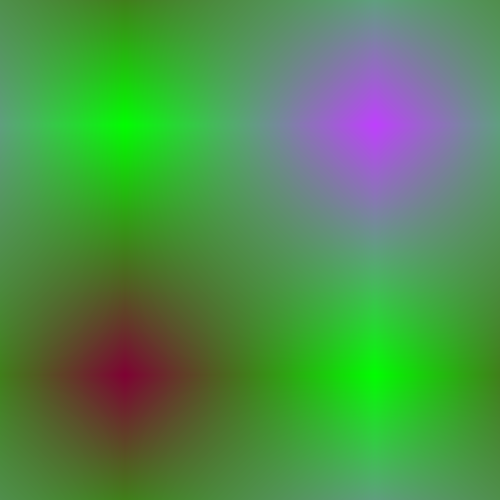
\includegraphics[width=4cm,height=4cm]{Figure4Bilinear.png}};
        \node[anchor=south west,inner sep=0] at (8.375cm,0.125cm) {
\includegraphics[width=4cm,height=4cm]{Figure4Curves.png}};
        % representative line for where the quadratic bezier curve lives
        \draw[yellow,->,line width=0.5mm]    (5.25cm,1.125cm) -- (7.25cm,3.125cm);    
        \draw (0.08,0.25) node[] {\Huge{A}};
        \draw (0.25,0.25) node[] {\Huge{B}};
        \draw (0.08,0.75) node[] {\Huge{B}};
        \draw (0.25,0.75) node[] {\Huge{C}};            
    \end{tikzpicture}
    \caption{Left: a 2x2 texture storing control points for a quadratic Bezier curve in each color channel.  Center: The same texture as viewed when using bilinear texture sampling.  The yellow line indicates where texture samples are taken from to evaluate the quadratic Bezier curve. Right: The curves resulting from sampling along the yellow line (Alpha curve ommited).}   
    \label{fig:texbilcurve}
  \end{figure}  

\subsection{Mathematical Basis}

TODO: this section.
TODO: show linear, bilinear, trilinear interpolation to be equivelant!  How to prove for N dimensions?

TODO: find where this text belongs.
While the Bernstein form of Bezier curves is equivelant to evaluating a Bezier curve with the De Casteljeau algorithm, in practice there are differences that come up between the two.  For instance, it is well known that the De Casteljeau algorithm is slower but more numerically robust than evaluating the Bernstein form.

The technique presented in this paper is no different.  While it's been shown that the multidimensional linear interpolation capabilities can be mathematically equivelant to the Bernstein form as well as the De Casteljeau algorithm, there are mathematical precision issues due to current GPU architectures.

TODO: give the details of the architecture and cite the two papers cited from the other place!

TODO: show accuracy in practice vs calculated in shader program.  Mention that it's "ok" in practice, better than standard texture baking, and reference the section that gives more information on this accuracy issue and how to improve it?

%-------------------------------------------------------------------------
\section{The Technique}
\label{sec:thetechnique}

While this technique is able to be used with any texture dimensionality, there are different characteristics when using textures of different dimensionalities.  Those characteristics will be explored here.

\subsection{One Dimensional Textures}

One dimensional textures are textures which have N pixels in a single row or column, such as 8x1, 16x1 or more generally Nx1.

Using one dimensional textures, the built in texture interpolation is only able to perform linear interpolation, which allows calculations of only 1st order (linear) Bezier basis functions.

That means that if you want a Bezier curve higher than order 1, you are going to have to take more texture samples and combine the results in the shader program.  While this is more expensive computationally, it does have the benefit of doing more of the work in the shader program, which has higher precision, so the end result will be a higher quality curve.

TODO: Flesh out details, show diagram of texture layout.
TODO: Maybe just GLSL for linear and quartic, but images for linear, quadratic, cubic, quartic with comparison vs "ground truth".


\subsection{Two Dimensional Textures}

Two dimensional textures are textures which are MxN pixels in size, such as 8x8 or 16x16 or 32x4.

Using two dimensional textures allows the texture interpolator to perform bilinear interpolation, which allows calculations of 2nd order (quadratic) Bezier basis functions.

If you want a Bezier curve higher than order 2, once again you are going to have to take more texture samples and combine the results in the shader program.  While more computationally expensive, it again results in higher precision results.

TODO: flesh out details, show diagram of texture layout.
TODO: GLSL for quadratric and quartic, but images for quadratic, cubic, quartic with comparison vs "ground truth".
TODO: explain how linear can still be achieved even if it isn't that useful (yet? Hw/sw)

\subsection{Three Dimensional Textures}

Three dimensional textures (often refered to as volumetric textures) are textures which are MxNxO pixels in size such as 8x8x2 or 16x8x4.

Using three dimensional textures allows the texture interpolator to evaluate trilinear interpolation, which allows calculations of 3rd order (cubic) Bezier basis functions.

Again, you can take more texture samples and combine the results in the shader program to get higher than order 3 curves if desired.

TODO: flesh out details, show diagram of texture layout.
TODO: GLSL for cubic and quartic, but images for cubic, quartic with comparison vs ground truth.
TODO: explain how linear and quadratic could still be achieved even if it isn't that useful (ye? Hw/sw)
TODO: beyond 3d textures? Could do 4d with mipmapped volumetric textures!

\subsection{Summary of Implications of Texture Dimensionality}

TODO: dimensionality / curve order comparisons. A table? Maybe side by side images?
TODO: texture size changes, number of textures used, number of texture samples taken
TODO: include quadrilinear and above?
TODO: we might want to do this in the performance results section instead and provide perf metrics as well.

%-------------------------------------------------------------------------
\section{Extensions}
\label{sec:extensions}

There are a few ways to extend this technique for more options.

\subsection{Combining Color Channels}

TODO: this.  Higher order curves without more texture reads

\subsection{Piecewise Curves}

TODO: this.  Pros and cons. B-splines can be converted to piecewise Bezier with Boem's algorithm (what's it called again?).

\subsection{Rational Bezier Curves}

TODO: this.
TODO: Nurbs can be converted to rational bezier curves with Boem's algorithm as well

\subsection{Multidimensional Bezier Curves}

TODO: this.  Each color channel is an axis.

%-------------------------------------------------------------------------
\section{Addressing Accuracy Issues}
\label{sec:addressingaccuracyissues}

TODO: this. HW vs SW vs HWSW hybrid vs read points yourself and do math w/o using interpolator. Everythign in between.
TODO: images to show differences.

%-------------------------------------------------------------------------
\section{Limited Applications for Vector Graphics}
\label{sec:limitedapplicationsforvectorgraphics}

TODO: this
TODO: mention that it isn't ideal since this technique is only good if you already know time "t" to evaluate, which is difficult to get otherwise.
TODO: mention that you don't have access to the control points since the interpolator does that level of math for you, but that affine transformations on the resulting curve point is equivelant to doing then on the control points.
TODO: mention 1d curve usage
TODO: mention polar curve usage
TODO: mention use for color gradients
TODO: picture of flag
TODO: put real usages here: particle properties, and whatever else.


%-------------------------------------------------------------------------
\section{Comparisons With Other Techniques}
\label{sec:comparisonswithothertechniques}

TODO: real apples to apples comparisons with texture baking (can be any order!) as well as shader constants.

%-------------------------------------------------------------------------
\section{Performance Characteristics}
\label{sec:performancecharacteristics}

TODO: Show some real performance values. 
TODO: show difference between 3d texture doing cubic, vs 2d texture with 2 texture reads and shader program results.
TODO: show results from multiple GPUs?

%-------------------------------------------------------------------------
\section*{Future Work}
\label{sec:futurework}

TODO: this

%-------------------------------------------------------------------------
\section*{Acknowledgements}
\label{sec:acknowledgements}
TODO: this


%-------------------------------------------------------------------------
\section*{References}
\label{sec:references}
TODO: this


%-------------------------------------------------------------------------
\section*{Index of Supplemental Materials}
\label{sec:indexofsupplementalmaterials}
TODO: this


%-------------------------------------------------------------------------
\section*{Author Contact Information}

\hspace{-2mm}\begin{tabular}{p{0.5\textwidth}p{0.5\textwidth}}
Roy G. Biv \newline
Colortech, Inc. \newline
29 Red Blvd. \newline
New York, NY 10511 \newline
\href{mailto:roy@colortech.com}{roy@colortech.com}
&

Raymond Trace \newline
Graphica University \newline
37 Rue De Lambert \newline
Paris, 75009 France \newline
\href{mailto:rtrace@graphica.edu}{rtrace@graphica.edu} \newline
\href{http://graphica.edu/~rtrace}{http://graphica.edu/\textasciitilde rtrace}

\end{tabular}


\afterdoc

\end{document}
